
\documentclass[final, fmstyle, lic]{tesis}

% paquetes usados
%\usepackage[chapter, spanish]{theorems}
\newtheorem{theorem}{Teorema}[chapter]
\newtheorem{lemma}{Lema}[chapter]
\newtheorem{proposition}{Proposición}[chapter]
\newtheorem{corollary}{Corolario}[chapter]
\newtheorem{definition}{Definición}[chapter]
\newtheorem{example}{Ejemplo}[chapter]
\newtheorem{observation}{Observación}[chapter]

\usepackage{symbols}
\usepackage{graphicx} %usar imágenes externas
\usepackage{url}
\usepackage{blindtext}
\usepackage[table,xcdraw]{xcolor}

\usepackage[utf8]{inputenc}  % descomentar para teclado en español de Unix, Mac y posiblemente Windows
\usepackage[T1]{fontenc} % this helps hyphenate Spanish vocabulary with acute accent
%\usepackage[latin1]{inputenc}  % descomentar para teclado en español de Unix y posiblemente también de Windows
%\usepackage[applemac]{inputenc}  % descomentar para teclado en español de Mac
\usepackage[spanish]{babel}
\decimalpoint

\setlength{\parskip}{2mm}	%Espaciado entre párrafos

\usepackage{hyperref}
%\usepackage{urm}
% datos de la tesis
\title{Sistema de monitoreo para estaciones meteorológicas}
\author{142912}{Teo González Calzada}
\authorb{}{}
\director{Mtro.}{José Fernando Estrada Saldaña}
\directorb{Dr.}{Felipe Adrián Vazquez Galvez}
\directorbp{«Profesor-Investigador IIT»}  % Dejar en campo en blanco si no hay segundo asesor
\sinodala{Dr.}{Nombre del Sinodal A}
\sinodalb{Dr.}{Nombre del Sinodal B}
\sinodalc{Dr.}{Nombre del Sinodal C}
\titular{Dr.}{Nombre del profesor de la materia} % Titular de Seminario de Titulación II

% comenta para automático:
\termyear{\today}

\begin{document}
\pagenumbering{roman}

\maketitle     % esto hace las portadas
\approvalpage  % esto hace la pagina de aprobaci√õn
\approvalprint  % esto hace la pagina de aprobaci√õn
%\approvalprint % esto hace la pagina de aprobaci√õn de impresión. Comentar si sólo un alumno
\originalpage

% Inicio de los Agradecimientos
\begin{thanks}

[Sustituye este texto escribiendo tus agradecimientos.
La sección de agradecimientos reconoce la ayuda de personas e instituciones que aportaron significativamente al desarrollo de la investigación. No te debes exceder en los agradecimientos; agradece sólo las contribuciones realmente importantes, las menos importantes pueden agradecerse personalmente. El nombre de la agencia que financió la investigación y el número de la subvención deben incluirse en esta sección. Generalmente no se agradecen las contribuciones que son parte de una labor rutinaria o que se reciben a cambio de pago. 

         Las contribuciones siguientes ameritan un agradecimiento pero no justifican la coautoría del artículo: ayuda técnica de laboratorio, préstamo de literatura y equipo, compañía y ayuda durante viajes al campo, asistencia con la preparación de tablas e ilustraciones o figuras, sugerencias para el desarrollo de la investigación, ideas para explicar los resultados, revisión del manuscrito y apoyo económico”.
]


\end{thanks}
% Fin de los Agradecimientos
\setcounter{page}{6}
% Inicio de Dedicatoria

\chapter*{Dedicatoria}

A mi padre, que ya no está conmigo, y a mi madre y hermana que lo están, por su apoyo incondicional durante todos estos años.

%! TODO, mejor redacción


% los siguientes comandos producen Ìndices.
% tablas y figuras en el documento de la tesis
\tableofcontents
\listoffigures
\listoftables

% Inicio de Resumen
\chapter*{Resumen}
\markboth{chapter name}{Sinopsis}

% [Sustituye este texto escribiendo tu sinopsis o resumen. Es un panorama general de todo lo que el lector encontrará en tu documento, en no más de una página. Recuerda que este, junto con el título, son la parte más leída de tu documento cuando alguien más lo busca en las bases de datos, el “punto de venta''.]

%! Oración en la que se describa con qué se construyó el sistema, o describir cuantas estaciones meteorológicas estan conectadas al sistema.

En el presente documento se reporta el desarrollo de un sistema de monitoreo de estaciones meteorológicas que también permite el control de las mismas. Este sistema fué probado durante 20 días monitoreando contínuamente el estado de las estaciones meteorológicas y ofrece la información recabada en una interfaz comprensible.

\textbf{Palabras clave}: Monitoreo de sistemas, Sistema integral, Desarrollo web.


\setcounter{page}{1}

\setcounter{page}{1}
\pagenumbering{arabic}
% Inicio de \section*{Introducción}\label{introduccion}
\chapter*{Introducción}\label{introduccion}

[Redacte de manera coherente en una cuartilla cuál es la nueva contribución, su importancia y por qué es adecuado para sistemas computacionales. Se sugiere para su redacción seguir los cinco pasos siguientes: 1) Establezca el campo de investigación al que pertenece el proyecto, 2) describa los aspectos del problema que ya han sido estudiado por otros investigadores, 3) explique el área de oportunidad que pretende cubrir el proyecto propuesto, 4) describa el producto obtenido y 5) proporcione el valor positivo de proyecto.]

% Las redes de monitoreo de calidad del aire de alta densidad son una necesidad creciente de las áreas urbanizadas. Estas permiten monitorear la calidad del aire a escala local, generando información vital para la toma de desiciones en áreas de salud pública. Al incrementar la cantidad de estaciones de monitoreo, la resolución de los datos aumenta, pero también aumentan el costo, la infraestructura y el personal necesario para atenderlas \cite{urban_air_quality}. De la misma forma, la demanda para redes de monitoreo climatológico de alta densidad ha ido en aumento por su utilidad en la medición de los impactos de las políticas de control en el ambiente \cite{muller_sensors_and_the_city}.

% Las instalaciones de monitoreo climatológico eran acostumbradas a ubicarse en las afueras de complejos ubranizados, centrados en la recolección de información para un análisis a escala global de los datos climatológicos, tales como el análisis del calentamiento global y los índices de radiación, así como otros datos importantes. Debido a los cambios en las necesidades de calidad y cantidad de datos, esto ha cambiado significativamente \cite{oke_2004}, y debido a ello, las redes de monitoreo de alta densidad se han convertido en un reto logístico y económico por resolver.

% Las estaciones de monitoreo climatológico funcionan de la misma forma que la mayoría de los servidores en el mercado; Un equipo de cómputo que está corriendo un servicio escucha constantemente las peticiones de los clientes a los que está conectado, creando y actualizando datos conforme es necesario. El equipo de cómputo además se conecta a sensores que utiliza para el monitoreo contínuo de datos, los procesa, y los almacena para su posterior análisis. Esto crea la posibilidad de crear e integrar sistemas de monitoreo de equipos de cómputo para el análisis de la salud de las estaciones.


\chapter{Planteamiento del Problema}

Las redes de monitoreo de meteorológico y de calidad del aire de alta densidad son una necesidad creciente de las áreas urbanizadas, las cuales necesitan de una infraestructura cada vez más compleja para su monitoreo y mantenimiento. Estas necesidades crecientes de infraestructura han generado una demanda creciente de recursos humanos, y la falta de homogeneidad entre las estaciones de monitoreo presentan retos a conquistar para proveer servicios cada vez más sofisticados. En este capítulo, se discutirá la importancia de la infraestructura de monitoreo y se explicarán los diferentes métodos de realizarlo que son utilizados actualmente para monitorear las estaciones meteorológicas, así como una propuesta de solución para los problemas que los sistemas tradicionales existentes presentan.

\section{Antecedentes}

El desplegar y mantener una red meteorológica urbana compone bastantes retos: Entre la creciente dificultad de crear sistemas de medición estandarizados que se adapten al siempre cambiante paisaje urbano; como la instalación de los equipos de medición y de guardado de datos en áreas que permitan acceso para mantenimiento y que sean seguros; y la dificultad de encontrar un punto de acceso a internet adecuado para transferir la información generada, el generar una red de monitoreo es una tarea extensa y compleja.

Debido a estos retos, la comunidad de monitoreo climatológico y meteorológico se ha enfocado en la creación de sistemas que sean más eficientes y económicos. Entre estos esfuerzos, se encuentra el amplio uso de dispositivos RaspberryPi como centro de recolección de datos de estaciones de monitoreo \cite{rpi_weataher_station}, tanto caseras como profesionales, con la ayuda de sistemas abiertos para la recolección de datos como lo es WeeWX. Esto ha hecho factible el desplegar redes de 50 nodos de monitoreo con sensores económicamente viables para actores con un presupuesto limitado \cite{monitoreo_raspberry_nagios}.

% TODO! Agregar sección de monitoreo de Campbell, y como funciona actualmente. Port forwarding en Campbell, porque no están en nuestra red.

%! Davis Weatherlink Live. https://www.davisinstruments.com/weatherlinklive/

Estas redes densas requieren de un monitoreo continuo para mantener una alta calidad de los datos recabados, y así evitar las pérdidas por falta de mantenimiento. Entre los sistemas de monitoreo que pueden ser adaptados para el monitoreo de estaciones meteorológicas y la red que las soporta, se encuentra la plataforma Nagios, la cual es un sistema de monitoreo continuo orientado a redes y servidores. Entre la información que recaba Nagios continuamente para el estado de los servidores, se encuentra el uso de CPU y RAM, así como estado de los discos, puertos, e información variada de servicios de red en los hosts. Debido a que Nagios es un sistema de monitoreo de redes orientado a profesionales de la informática, la interfaz gráfica es poco amigable con los usuarios menos familiarizados con los conceptos técnicos de los sistemas computacionales, como se muestra en la Figura \ref{fig:nagios_dashboard}.

\begin{figure}[!ht]
	\centering
	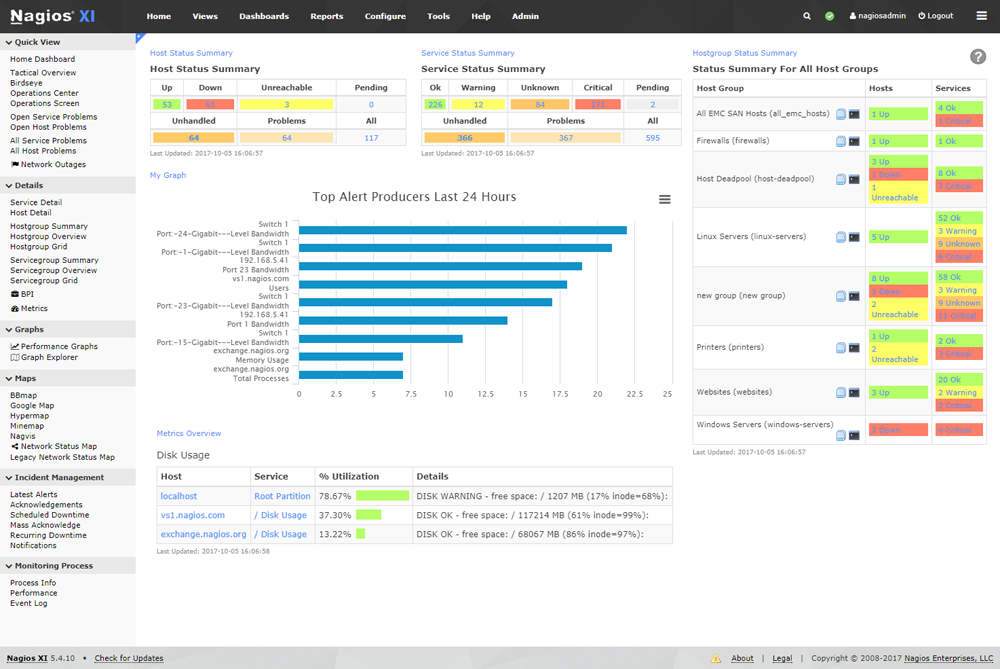
\includegraphics[width=1\linewidth]{images/Nagios_home_dashboard.png}
	\caption{Tablero principal de Nagios XI.}
	\label{fig:nagios_dashboard}
\end{figure}

Nagios ofrece la posibilidad de monitorear parámetros adicionales y posee una comunidad establecida que desarrolla continuamente en diversos lenguajes, como Python, un sistema conformado por plugins relacionados con el proyecto. Sin embargo, la cantidad de éstos relacionados con estaciones meteorológicas existentes es mínima ya que los esfuerzos de la comunidad se centran principalmente en el monitoreo de centros de datos, redes y routers.

Además de los plugins existentes en la comunidad de Nagios, existe la alternativa abierta conocida como \textit{monitoring plugins} \cite{monitoring_plugins}, que es una plataforma compatible con diversos sistemas de monitoreo de redes y servicios, en la cual es posible encontrar una mayor cantidad de scripts de monitoreo relacionados con los sistemas de recolección de datos meteorológicos. La utilización de estos \textit{plugins abiertos} junto con un sistema central como Nagios ya ha sido propuesto anteriormente, sin embargo, se descartó un monitoreo más profundo debido a que \say{las métricas obtenidas son muy simples y los valores se devuelven de comandos directos de sistema de GNU/Linux} \cite{monitoreo_raspberry_nagios}.

Las limitaciones de Nagios vienen a raíz de su implementación orientada a sistemas de alta disponibilidad y el generalismo en la implementación de monitoreo, la configuración de los parámetros de tolerancia para la resilencia a fallas son generalmente limitados en la variedad de los mismos y los valores fijos que se pueden establecer. Además, debido a las necesidades de seguridad y accesibilidad de las estaciones meteorológicas en el contexto urbano, estas suelen instalarse en sistemas en los que se posee poco control de la red que les provee comunicación, como son las escuelas, hospitales y estaciones de policía, así como otros espacios públicos \cite{muller_sensors_and_the_city}, dificultando aún más la capacidad de monitoreo y disponibilidad de la red y los sistemas que soporta. Esta limitante se hace más presente debido a que los sistemas se vuelven completamente dependientes de una VPN para funcionar y para su control, debido al extenso uso de redes IPv4 bajo NAT que predominan en los sitios de instalación.

Otra de las restricciones del sistema Nagios es que al ser un sistema de monitoreo limita la capacidad de acción de los usuarios ante un caso que lo requiera. Si bien es posible el realizar acciones por medio de scripts creados al momento de la configuración de Nagios, estos requieren una configuración extensa y compleja \cite{nagios_service_restart}. Además, el sistema basado en eventos impide la interacción directa de un usuario para la respuesta de forma directa desde la consola de administración, requiriendo que el usuario tenga un conocimiento del método de conexión, así como la información necesaria para realizar una tarea trivial como es el reiniciar un servicio.

Actualmente, el sistema de monitoreo de calidad del aire y climatológico del Centro de Ciencias Atmosféricas y Tecnologías Verdes (CECATEV) en la Universidad Autónoma de Ciudad Juárez, engloba varios de los retos antes descritos, ya que a pesar de la baja densidad de estaciones meteorológicas, comprende una variedad importante de las mismas. Esta compuesta por prototipos conectados por medio de redes virtuales privadas, monitoreados remotamente \cite{red_climatologica_uacj}, estaciones de diferentes proveedores, siendo monitoreadas local y externamente, así como estaciones remotas con routers dentro de la red local de la universidad (véase la Figura \ref{fig:current_network}). Lo que provoca que sea un reto monitorearlas adecuadamente debido a la variedad de sus componentes.

%* Los puertos no están expuestos si la conexión se realiza por NAT.

%! (Centro de Ciencias Atmosféricas y Tecnologías Verdes)

\begin{figure}[!ht]
	\centering
	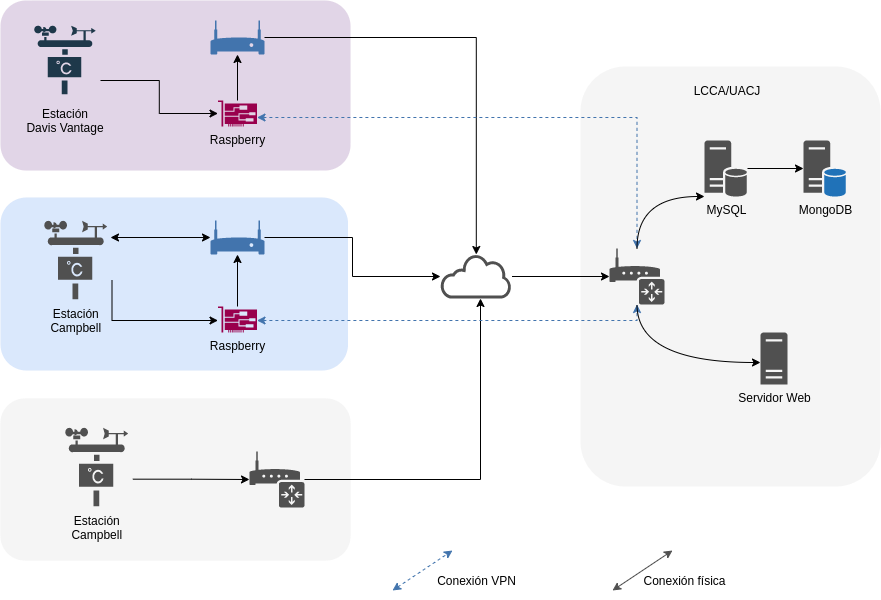
\includegraphics[width=.80\linewidth]{images/diagrams/red_lcca.drawio.png}
	\caption{Diagrama de red de CECATEV UACJ.}
	\label{fig:current_network}
\end{figure}

Desafortunadamente, la infraestructura de la red actual de CECATEV no cuenta con un sistema de monitoreo para el registro automático de problemas de las estaciones meteorológicas de la cual pueda ser derivada información de la calidad de los datos meteorológicos así como un estado de salud de las estaciones. Esto, dificulta el uso de forma adecuada de la información existente e impide la generación de reportes de calidad de la información.

\section{Definición del problema}

La falta de una plataforma estandarizada para el monitoreo de estaciones meteorológicas que permita un monitoreo continuo y control de diversos tipos de estaciones, así como la disponibilidad del acceso a los datos, y un registro de incidentes crea una dificultad creciente para los administradores de redes de monitoreo meteorológico. Con redes cada vez más densas que son más accesibles económicamente y menos complejas de crear, se hace notar la necesidad de un sistema estandarizado y compatible con soluciones existentes para el monitoreo de las estaciones.

\section{Objetivo general}

Desarrollar un sistema de monitoreo y control de estaciones meteorológicas para personal no especializado, capaz de proveer datos y herramientas que coadyuven en el mantenimiento preventivo y correctivo de las mismas.

\subsection{Objetivos específicos}

\begin{itemize}
   \item Desarrollar un sistema modular central para coordinar y recolectar los datos del estado de las estaciones.

   \item Diseñar un API REST para consultar el estado de las estaciones meteorológicas.

   %! Agregar como subobjetivo una base de conocimientos. (como lo justifico?) Demostrar tiempos de respuesta para QAPP.
   %! Herramientas de gestión de calidad
   %! Personas como parte de gestion

   \item Diseñar e implementar una interfaz gráfica para monitorear el estado de las estaciones.

   \item Integrar las diferentes estaciones meteorológicas existentes al sistema creando los controladores correspondientes.

   \item Integrar un sistema existente de notificaciones/alertas de terceros para fallos críticos de las estaciones.
\end{itemize}

\section{Justificación}

Creando un sistema de monitoreo eficaz para las estaciones meteorológicas se pretende alcanzar una mayor calidad de los datos obtenidos de las mismas, así como una mejor documentación por consecuencia de los problemas de los sistemas meteorológicos. Lo cual permitirá dar el tiempo al personal especializado en enfocarse en expandir las redes existentes meteorológicas, mejorando a largo plazo la calidad y la definición de los datos recabados con la misma cantidad de esfuerzo.

Además, haciendo el sistema de monitoreo un proyecto público y compatible con soluciones existentes, se busca ayudar a mejorar la calidad y confiabilidad de las redes de monitoreo meteorológico, de calidad del aire y climatológico alrededor del mundo.

Este proyecto tiene un impacto tecnológico, debido a que se plantea desarrollar un sistema en el que se puedan integrar diversos datos que ayuden a generar un estado comprehensible de la calidad de la información de las redes meteorológicas que monitorea. Con respecto al impacto económico, el proyecto permitirá identificar y solucionar los problemas que pudieran ocurrir en las diferentes estaciones sin la  necesidad de desplazarse para corregir la solución, propiciando un uso más eficiente de los recursos humanos y económicos de CECATEV cuyo financiamiento principal para la operación son recursos públicos.

El impacto ecológico del proyecto es indirecto, ya que el personal de CECATEV podrá dedicar mayor tiempo al tratamiento de la información generada por las estaciones y no en desplazarse a las diferentes estaciones para identificar los problemas y solucionarlos.

\section{Alcances y limitaciones}

\noindent Entre los alcances que se pretendían lograr con el proyecto, se contemplaron los siguientes:

\begin{itemize}

   \item Se integraron estaciones meteorológicas existentes, que se encontraban conectadas a la red de comunicaciones del CECATEV ya sea directamente o por medio de una VPN.

   \item Se entregó un sistema instaldo, funcional y listo para monitorear las estaciones seleccionadas, sin necesidad de configuraciones extraordinarias.

\end{itemize}

Si bien se pretende que el proyecto tenga la flexibilidad suficiente para adaptarse a nuevos casos de uso sin necesidad  de reescribir grandes partes del mismo, también se consideran las siguientes limitaciones:

\begin{itemize}

\item La integración se limitó a cubrir casos conocidos y recurrentes de estaciones meteorológicas existentes.
\item Solo se considera integrar una estación meteorológica de cada tipo en cada topología, dejando como proyecto futuro integrar la totalidad de la red de la universidad.
\item El sistema se limita a cubrir los casos de fallas comunes y conocidos de las estaciones.
\item Sólo se monitorean los servicios básicos de las estaciones meteorológicas que son vitales para el funcionamiento.
\end{itemize}

\chapter{Marco referencial}

%! Párrafo introductorio abajo de la frase marco referencial



\section{Marco teórico}

% [Es la selección, exposición y análisis de la o las teorías, métodos, procedimientos y conocimientos que sirven para fundamentar el tema, explicar los antecedentes e interpretar los resultados de la investigación. La teoría constituye la base donde se sustentará cualquier análisis, experimento o propuesta de desarrollo de un trabajo de grado.]

% Aqui se presenta la información general, en el desarrollo se pone cómo se usó la información.

% \subsection{Estación meteorológica}


% Automatic weather stations

% %! Agregar un tema general

% \subsection{Redes meteorológicas}

% \subsection{Redes de comunicación}

% Red Local, redes NAT y capas de NAT en el pais. Mencionar direcciones públicas

% \subsection{Modelo OSI}

% \subsection{VPN}

% Seguridad de la información

% Protocolo SSH y (Network monitoring)

% VPN (Incluir segmento sobre a seguridad involucrada en la VPN), y sobre la facilidad de conexion con SSH


% \subsection{API REST}

Los sistemas informáticos que se componen de más de un componente, utilizan diversos métodos de comunicación entre ellos. Desde el accesar directamente a localizaciones de memoria física o virtual en un dispositivo para compartir información hasta crear librerías compartidas entre sistemas para accesar a la información en un depósito externo (conocidas como APIs), cada forma de acceso a los datos tiene su propio nivel de abstracción, oportunidades, y desventajas, las cuales deben ser evaluadas antes de elegir una tecnología adecuada para responder a las necesidades de cada proyecto.

%! Bibliotecas de software, no bibliotecas
%! ¿Cambiar el término de API por interfaces? (A menos que las interfaces estén en bibliotecas).

Un API REST es un estándar de acceso a la información de sistemas externos por medio de protocolos \textit{Web}, tales como HTTP/HTTPS, los cuáles permiten la consulta de datos en cualquier lenguaje que permita realizar conexiones y consultas a sitios web \cite{REST_API_design}. Entre las principales características de los API REST se encuentra que no es necesario proveer un estado previo para acceder a la información, esto implica que no es necesario mas que conocer la ruta en la que se encuentran los datos requeridos para acceder a ellos. Las ventajas que ofrece es la amplia disponibilidad de acceso a los datos y la fácil integración con sistemas existentes de manejo y procesamiento de información \cite{OpenAPI_example}.

%! Mencionar esta figura!!

\begin{figure}[!ht]
	\centering
	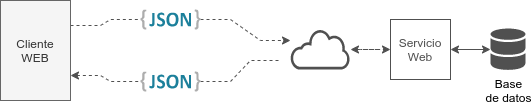
\includegraphics[width=.70\linewidth]{images/diagrams/REST.png}
	\caption{Diagrama del protocolo REST.}
	\label{fig:coms_nodos_raspberry}
\end{figure}

% \subsection{OpenAPI}

Debido a la naturaleza libre de el desarrollo web, y la poca estandarización de la comunicación entre los clientes web con los servidores, se creó la iniciativa OpenAPI a partir de un estándar existente proveído por la compañía Smartbear, Swagger. Este estándar para la comunicación con sitios por medio de APIs REST rápidamente fué ganando popularidad gracias a la fundación Linux hasta convertirse en un estándar utilizado ampliamente por diversas organizaciones y empresas \cite{OpenAPI_foundation}.

El estándar OpenAPI es un esquema de definición de estructura de datos en JSON. En este esquema se definen las rutas a las cuáles se puede acceder, los parámetros que aceptan y sus respectivos tipos de datos, así como la información que responde y los tipos de datos de los mismos. Y debido a la naturaleza abierta del esquema, este puede ser generado e integrado nativamente con el uso de diversas tecnologías de desarrollo. Permitiendo, por ejemplo, el generar las clases e interfaces correspondientes para el uso por medio de clases de los datos para lenguajes de programación fuertemente tipados \cite{openapi_generator}.

% Configuración de los archivos, del docker, la forma en la que está configurado el sistema, importar paquetes de python

\section{Marco Conceputal}

Estaciones climatologicas

Una estación climatológica es un sistema de medición de la temperatura, humedad, presión, velocidad del viento, etc. que se encuentra en una ubicación determinada.

Tipos de estaciones: Campbell, RaspberryPI, Arduino, etc.

WeeWX, VPN, NAT, etc.

Diagrama de la red UACJ

\section{Marco tecnológico}

%! Desarrollar el marco tecnológico.
%! Desarrollar marco tecnológico, con imágenes y etc.

%! Aplicaciones, capacidades, performance, etc

A continuación se presenta una descripción de las herramientas de tecnología que se utilizarán para el desarrollo del proyecto.

\subsection{Docker}

Docker es un sistema para la creación y distribución de imágenes de software, principalmente orientado a servidores, que permite el crear un ambiente replicable agnóstico al sistema operativo del host. Es un estándar en la industria de desarrollo de software para crear sistemas complejos manteniendo una relativa simpleza al desplegar nuevas instancias \cite{rad2017dockerAnalysis}.

%* Palabra figura

Docker utiliza un sólo Kérnel de linux para la creación de los contenedores y cada uno de los contenedores puede contener hasta \textit{n} procesos, lo que lo ayuda a reducir el tamaño de sistemas complejos como se muestra en la Figura \ref{fig:docker_diagrama}. Además de ofrecer una mayor flexibilidad y escalabilidad para tanto para realizar pruebas en máquinas de desarrollo como para distribuir y empaquetar nuevas instancias en ambientes de producción, se ha demostrado que el costo en eficiencia al sistema que lo ejecuta es mínimo comparado con otros métodos para la administración de sistemas complejos tales como las máquinas virtuales y el empaquetado en KVM \cite{rad2017dockerAnalysis, felter2015comparsionPerformance}.

\begin{figure}[!ht]
	\centering
	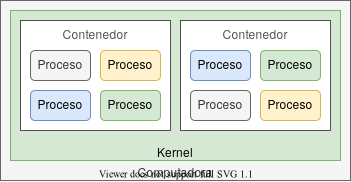
\includegraphics[width=.45\linewidth]{images/diagrams/docker.png}
	\caption{Diagrama del contenedor de procesos Docker.}
	\label{fig:docker_diagrama}
\end{figure}

\subsection{Masonite ORM}

Masonite ORM es una solución creada para python que permite la manipulación de sistemas relacionales de bases de datos creando una interfaz de código. Abstrae la complejidad de la manipulación de base de datos para convertirla en un modelo de clases con una interfaz simple para la edición de los datos. Tiene soporte nativo para transacciones, es compatible con MariaDB y está diseñado para ser incluido en proyectos complejos sin necesidad de incluir un framework completo \cite{masonite_2021}.

\subsection{FastAPI}

FastAPI es un framework para desarrollo de APIs REST para Python centrado en el desarrollo rápido con ayuda de las anotaciones estándar de Python. Además de ser uno de los frameworks de desarrollo más rápidos en su ejecución, permite el crear directamente documentación compatible con el estándar OpenAPI sin necesidad de librerías externas \cite{fastapi_ramirez_2020}. Todo esto lo convierte en un framework ideal para extender proyectos existentes en Python y con su permisiva licencia permite %* terminar esta oración

\subsection{MariaDB}

%! Quitar esto de aquí, cambiar a la selección de base de datos.

MariaDB es un motor de base de datos relacional creado por el equipo original que desarrolló MySQL, es un motor que tiene como objetivo mantenerse completamente abierto y tiene una licencia de uso permisiva para su uso en ambientes comerciales y no comerciales \cite{mariadb_foundation_2019}. Tiene un rendimiento similar a MySQL en operaciones transaccionales, por lo cual es una excelente alternativa cuando se requiere un modelo de licencias permisivo \cite{mariadb_comparison}.

%  TODO: Consider the use of a time series database.f

% TODO \subsection{React} Sección de tecnología para front, probablemente React

% SNM (Simple management network)
% OpenSource
% RaspberryPI
% Icinga

\chapter{Desarrollo del Proyecto}
[Este capítulo se considera el más importante al elaborar el proyecto de titulación. Se describe el procedimiento seguido para lograr el objetivo planteado. Se explica qué y cómo se hizo, además se debe de convencer de que los métodos o procedimientos usados fueron los más adecuados.

Deben detallarse los procedimientos, técnicas, métodos, metodologías y demás estrategias metodológicas requeridas para el proyecto.
]

\section{Producto propuesto}

Se propone crear un proyecto que permita monitorear el estatus de los servicios de las estaciones meteorológicas, y por **consiguiente** de la infraestructura en la que dependen, así como ofrecer un control limitado para la solución de problemas de forma remota.

El proyecto consistirá de tres partes independientes:

\begin{itemize}
   \item Un módulo para el monitoreo de el estatus de las estaciones, que permita el cargar la información de las estaciones de una base de datos, para luego cargar los controladores específicos de cada estación basado en la infrormación existente de las mismas para después guardar el estado en el que se encuentran en una base de datos.

   \item Un API REST que tendrá el objetivo de proveer un acceso sencillo a la información de los sistemas de monitoreo, así como el de proveer una interfaz de control para las estaciones que permita la ejecución remota de comandos preestablecidos, desde cualquier punto con la autorización adecuada que haga una petición a la ruta correspondiente.

   \item Una interfaz gráfica, que permita el acceso a la información correspondiente de los sistemas de monitoreo, así como acceso a los reportes que se generen y permita capturar informes de solución de problemas de las estaciones para su posterior análisis.

\end{itemize}

\section{Fases (Metodología)}

Para el desarrollo de este programa, se utilizará la estrategia de desarrollo ágil centrada en el usuario. En ella se combina la metodología de desarrollo ágil, la cuál tiene como características principales la entrega continua de resultados y la preferencia de sistemas funcionales sobre documentaciones de código robustas \cite{agile_manifesto}, con el diseño centrado en el usuario, el cuál tiene a los usuarios como objetivo principal para satisfacer las necesidades de requerimientos.

Debido a que la experiencia de usuario es uno de los factores que pueden separar al sistema en desarrollo de los sistemas actuales de monitoreo para equipos de cómputo, el esquema de entregas, desarrollo y planeación estarán centrado en el mismo \cite{hussain_agile_usercentered}. El ciclo de entregas será con un sprint de máximo dos semanas, para una revisión de las metas, planeación y objetivos a alto nivel con el usuario y redifinir los requisitos y como sea necesario. La documentación para el usuario final, así como la documentación del API y la información técnica del sistema será un producto que será entregado al finalizar el mismo, apoyándose de la información generada en los sprints.

En el respecto del lenguaje de programación, tomando en consideración que la red de monitoreo actual utiliza WeeWX para su integración con estaciones meteorológicas \cite{red_climatologica_uacj}, así como otros componentes del sistema de monitoreo existente, se pretende utilizar Python como lenguaje principal para el desarrollo del núcleo del sistema, sus módulos, y el API de consulta. Para el desarrollo de la interfaz gráfica del sitio web, se elegirá un framework ligero con Javscript. Todo esto se empaquetará en una imagen de Docker para permitir la replicación de la instancia con el mínimo esfuerzo posible.

\section{Programa de Actividades}

{\fontfamily{lmss}\selectfont
Se pretenden llevar a cabo las actividades de acuerdo al siguiente diagrama:

\begin{table}[h]
   \centering
   % \resizebox*{!}{12 cm}{
   \begin{tabular}{|p{9cm}|c|c|c|c|c|c|c|c|c|c|}
      \hline
      ACTIVIDAD&\rotatebox{90}{Febrero 2021}
      &\rotatebox{90}{Marzo}
      &\rotatebox{90}{Abril}
      &\rotatebox{90}{Mayo}
      &\rotatebox{90}{Junio}
      &\rotatebox{90}{Julio}
      &\rotatebox{90}{Agosto}
      &\rotatebox{90}{Septiembre}
      &\rotatebox{90}{Octubre}
      &\rotatebox{90}{Noviembre 2021}\\
      \hline
      Revisión de la Literatura& \checkmark & \checkmark  & \checkmark  &  &  &  &  &  & &  \\
      \hline
      Protocolo&\checkmark &\checkmark  &\checkmark  & \checkmark &  &  &  &  & &  \\
      \hline
      Selección de herramientas & &\checkmark  & \checkmark &  &  &  &  &  & &  \\
      % \hline
      % Documentación de propuesta&  &  & \checkmark & \checkmark &\checkmark  &\checkmark  &\checkmark  &\checkmark  &\checkmark  &\checkmark  \\
      \hline
      Diseño de la interfaz de usuario &  & \checkmark &  &  \checkmark & \checkmark &  &  &  &  &  \\
      \hline
      Documentación de requerimientos &  & \checkmark & \checkmark &  \checkmark & \checkmark &  &  &  &  &  \\
      \hline
      Diseño de la base de datos&  &  &  & \checkmark & \checkmark &  &  &  &  &  \\
      \hline
      Desarrollo del núcleo del sistema&  &  &  &  & \checkmark & \checkmark &  \checkmark &  &  &  \\
      \hline
      Desarrollo de la interfaz de usuario &  &  &  &  &  & \checkmark & \checkmark &  &  &  \\
      \hline
      Desarrollo e implementación del API REST&  &  &  &  &  & \checkmark & \checkmark & \checkmark &  &  \\
      \hline
      Integración con sistema de notificaciones &  &  &  &  &  &  & \checkmark & \checkmark &  &  \\
      \hline
      Compilación y entrega de documentación&  &  &  &  &  &  &  &  & \checkmark & \checkmark \\
      \hline

      Presentación y defensa de trabajo&  &  &  &  &  &  &  &  &  & \checkmark  \\
      \hline
   \end{tabular}
	\label{Cronograma}
   \caption{Actividades a diez meses}
\end{table}
}

%! Agregar octubre para la evaluación del instrumento.

\section{Selección de base de datos}

% Casi todas las secciones de desrrollo, van ligadas a una de resultados.

Con un tiempo de respuesta de $~[N]ms$, el sistema puede soprotar hasta N estaciones concurrentes.

Debido a que la recolección de los datos es por métodología pull y no push, es posible tener las estaciones en una cola que se ejecute hasta por un periodo de 5 minutos (que es un estándar en la recolección de datos de estaciones meteorológicas). Esto implica que la base de datos [X] puede soportar hasta [N x 60 x 5] datos de forma concurrente.

Tomando en cuenta las necesidades actuales del LCCA, y el estimado del tamaño de las redes de alta densidad (que pueden llegar hasta los N nodos como X artículo lo demuestra), no vale la pena el introducir la complejidad extra de un motor de base de datos desconocido y para el que no existen ORM's con soporte completo en el lenguaje de desarrollo. Porque no es un sistema de alta densidad de datos.

Si bien es posible escalar horizontalmente la infraestructura, se busca evitarlo ya que los diminishing returns del costo de tener que mantener un sistema de monitoreo no es costeable. Para los casos de sistemas de extremadamente alta densidad, se recomienda el crear varias instancias seccionadas en bases de datos, o escalar la base de con un redis en vez de escalar.

%! Recordar que la información debe ser consultada desde el API, así que no sólo se tienen que tomar en cuenta la cantidad de query's por segundo que se requieren hacer para las inserciones, sino también para la consulta de datos.

%! Si lo que queremos es proveer herramientas para la gestión de calidad de los datos meteorológicos, la información tiene que tener en mente los principios Solidos y transaccionales, al menos en la creación de reportes basados en incidentes.

\section{Diseño de base de datos}

\section{Avances}


\section{Módulo de monitoreo}

\subsection*{Requisitos}

\subsection*{Seguridad}

\subsection*{Método de conexion}


\chapter{Resultados y Discusiones}
% [En este capítulo se presentan los resultados obtenidos correspondientes al proyecto descrito en el capítulo anterior. Los resultados se pueden presentar en tablas o gráfica y deben ser redactados y organizados de tal manera que sea fácil de comprender por los lectores.

% La los resultados no se explican por si mismo, por lo que es necesario una discusión que los explique y muestre cómo ayudan a resolver el problema definido en el capítulo 1. La discusión puede mencionar someramente los resultados antes de discutirlos, pero no debe repetirlos en detalle. No prolongues la discusión citando trabajos ``relacionados'' o planteando explicaciones poco probables. Ambas acciones distraen al lector y lo alejan de la discusión realmente importante. La discusión puede incluir recomendaciones y sugerencias para investigaciones futuras, tales como métodos alternos que podrían dar mejores resultados, tareas que no se hicieron y que en retrospectiva debieron hacerse, y aspectos que merecen explorarse en las próximas investigaciones.]
%! Vaciar los datos,

Durante la fase de evaluación del sistema, este estuvo recolectando información de las diversas estaciones meteorológicas instaladas en la región. Esta información permite el evaluar la vaibilidad del proyecto a corto y mediano plazo, además de facilitar el realizar un análisis preeliminar de los datos recolectados. En la primer sección de este capítulo, se analizarán los datos recolectados por el sistema, posteriormente, se hará un análisis de la capacidad de extensibilidad del sistema para cubrir nuevos casos de uso y se terminará en pruebas de estrés y carga realizadas al mismo.

\section{Sobre los datos obtenidos}

Gracias a la información recabada durante el periodo de evaluación del sistema, fue posible el realizar un análisis preeliminar de los datos recolectados de las estaciones. Dentro de estos datos se encuentra los tipos de incidencias, su duración y la fecha en la que estas ocurrieron, así como datos diversos específicos por cada tipo de incidencia.

Al revisar la información recolectada, se encontró que el mayor problema que se presenta en las estaciones es la inaccesibilidad por red a las mismas, como puede observarse en la figura \ref{fig:station-errors-by-type}. Esta falta de comunicación con las estaciones puede deberse a una serie de factores, como una conexión deficiente de red, problemas temporales del servicio de VPN con el que cuentan las estaciones, o falta de energía en el dispositivo.

\begin{figure}[!ht]
   \centering
   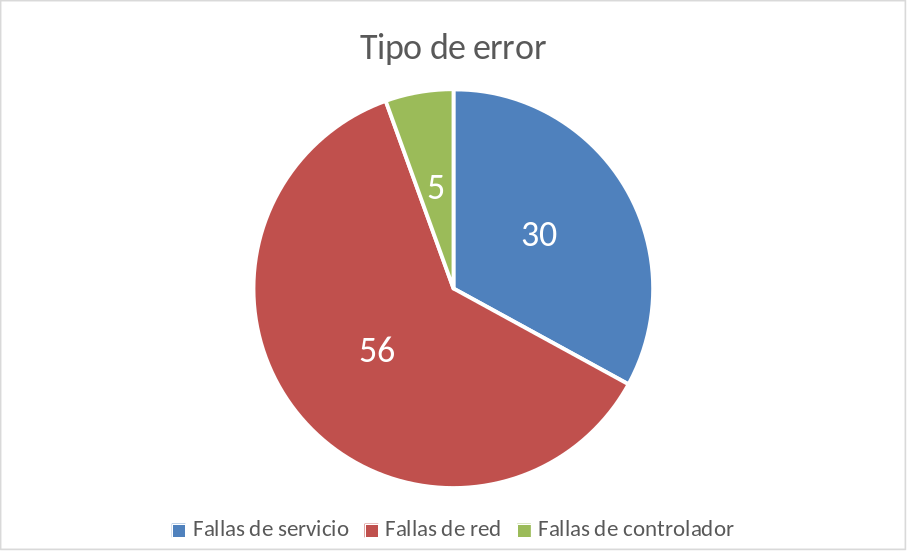
\includegraphics[width=0.7\linewidth]{images/graphs/by_type.png}
   \caption{Tipos de incidencia.}
   \label{fig:station-errors-by-type}
\end{figure}

Como se muestra en la Figura \ref{fig:station-incidents}, el número de incidentes es dependiente de cada estación, esto implica que no existe una coorelación entre ellas. Además, al compararlo con los datos obtenidos de la Figura \ref{fig:cumulated-downtime}, es posible observar que el número de fallas de red es directamente proporcional al tiempo de indisponibilidad de cada estación.

\begin{figure}[!ht]
   \centering
   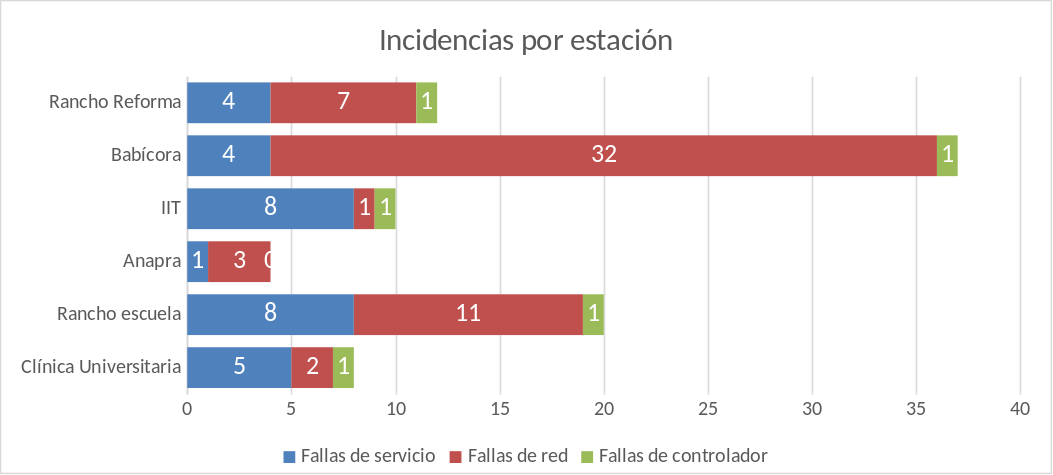
\includegraphics[width=0.9\linewidth]{images/graphs/by_station_incidents.png}
   \caption{Incidencias y sus tipos, agrupadas por estación.}
   \label{fig:station-incidents}
\end{figure}

\begin{figure}[!ht]
   \centering
   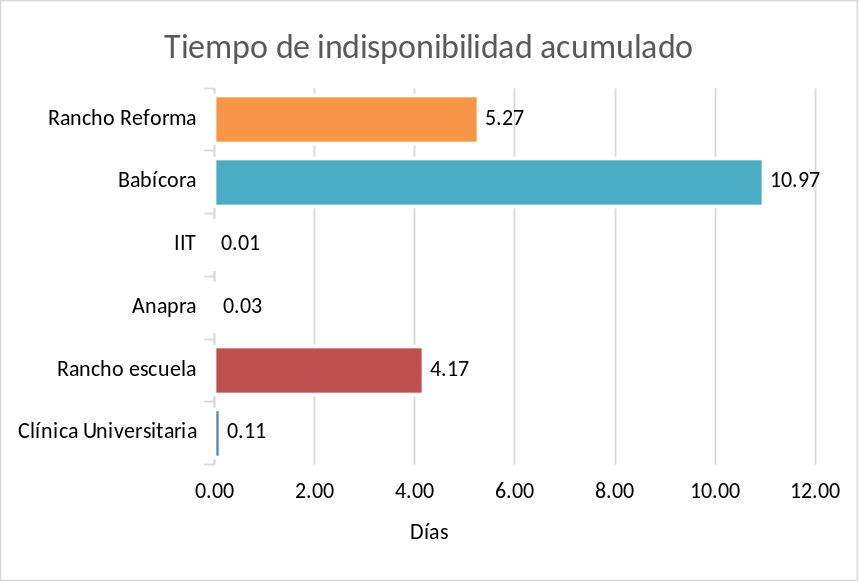
\includegraphics[width=0.65\linewidth]{images/graphs/cumulated_downtime.png}
   \caption{Tiempo de inaccesibilidad acumulado por estación.}
   \label{fig:cumulated-downtime}
\end{figure}

También, es posible observar que la falla que permaneció activa por más tiempo es un error en la base de datos MySQL que impedía el correcto almacenamiento de la información recabada por la estación. La pérdida de estos datos se puede verificar en la página de monitoreo de los datos generados de la estación en la Figura \ref{fig:rancho-data-loss} en la forma de ausencia de información en gráfica de la vista semanal de los sensores.

\begin{figure}[!ht]
   \centering
   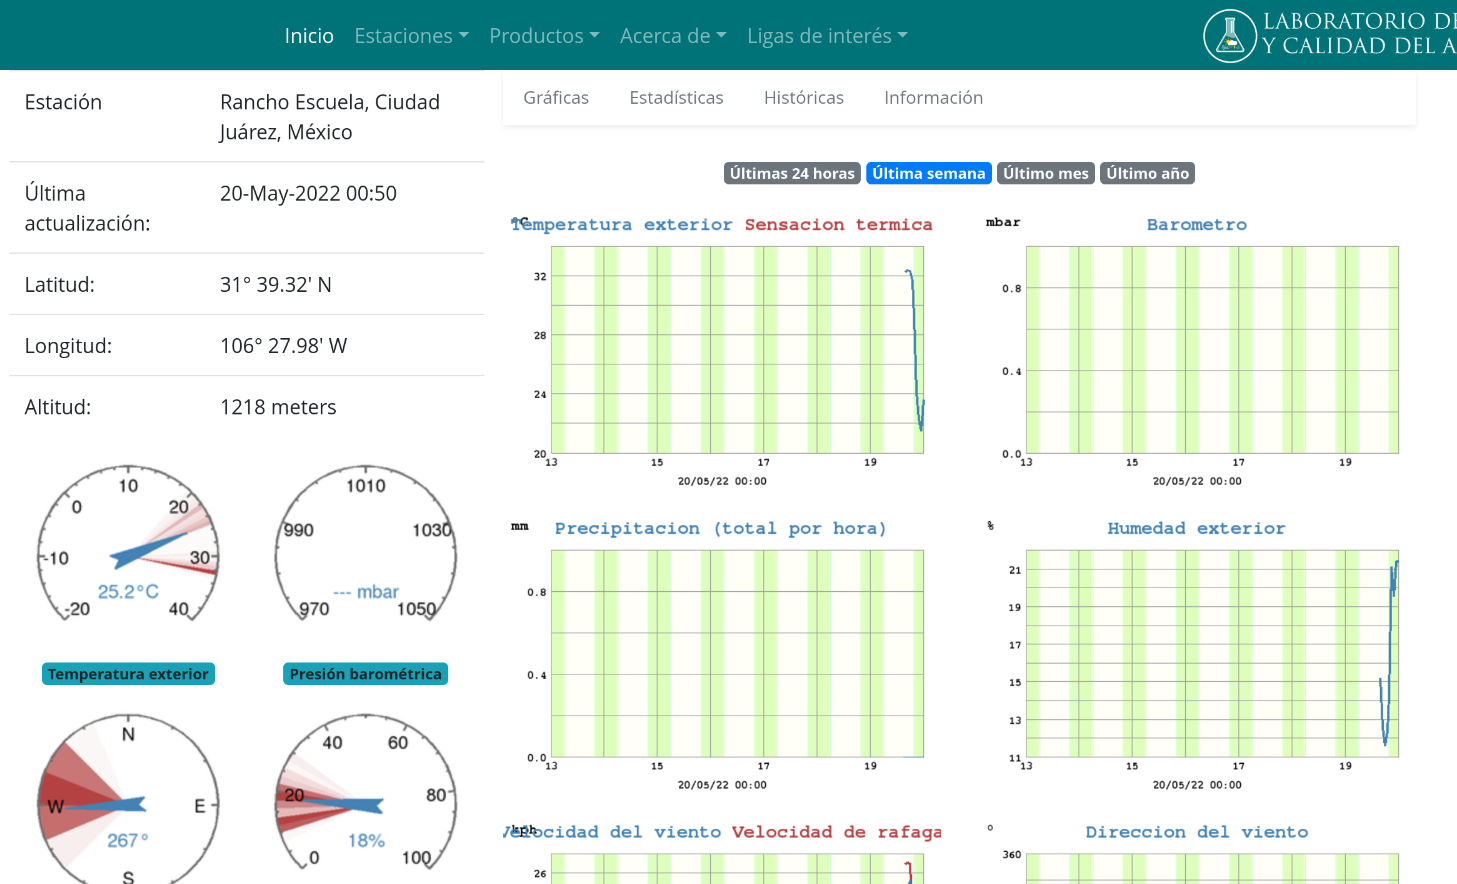
\includegraphics[width=1\linewidth]{images/screenshots/rancho-data-loss.png}
   \caption{Rancho escuela.}
   \label{fig:rancho-data-loss}
\end{figure}

El error de recolección de la información fue resuelto, y la fecha de solución, como se muestra en la Figura \ref{fig:rancho-data-solved}, coincide con la pérdida de datos de la estación. Esto permite realizar una coorelación de una falla concreta de una estación con la pérdida de información. Esta información, puede ayudar al personal de CECATEV a realizar un proceso de mejora contínua para la evaluación y categorización de fallas de las estaciones, con el objetivo de priorizar los fallos que afectan la calidad de los datos como tarea fundamental.

\begin{figure}[!ht]
   \centering
   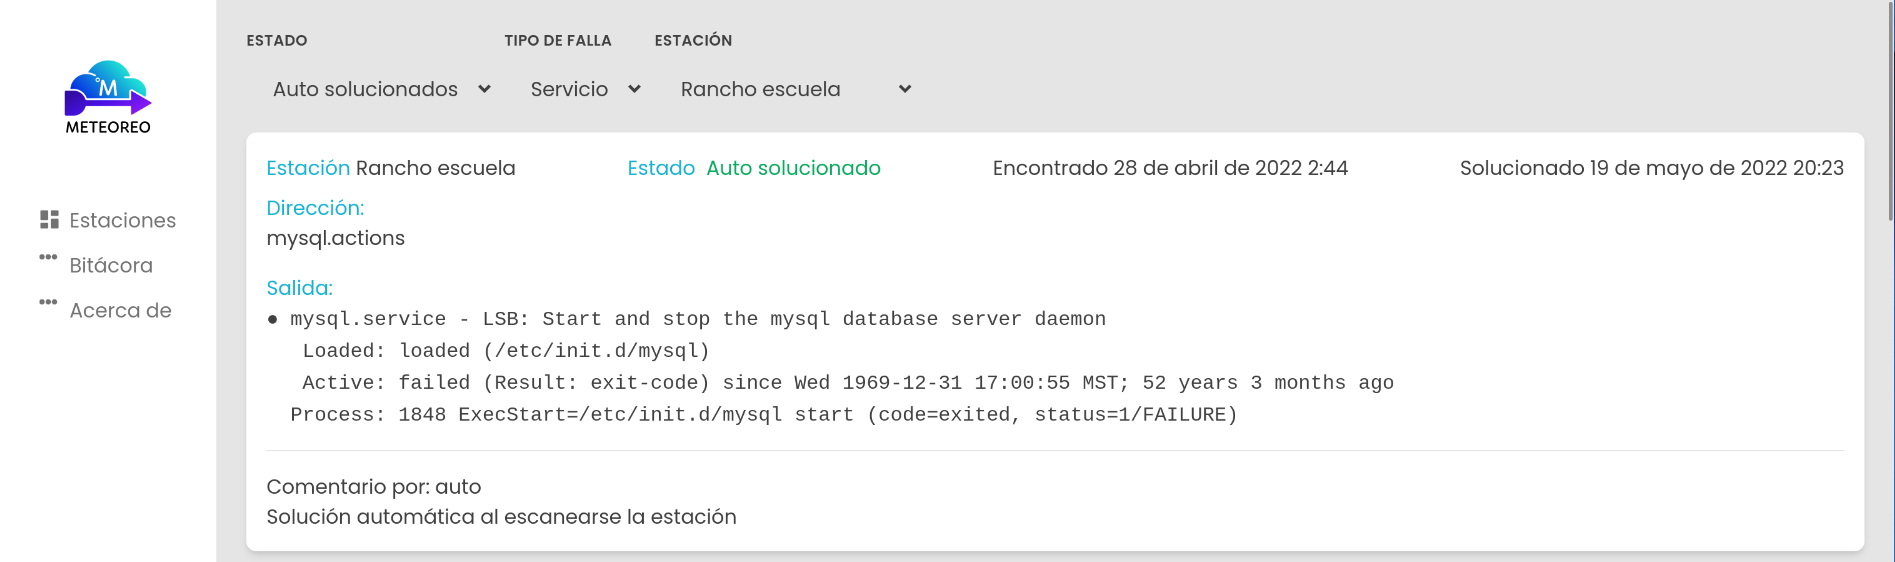
\includegraphics[width=1\linewidth]{images/screenshots/rancho-mysql-solved.png}
   \caption{Datos de falla de Rancho Escuela.}
   \label{fig:rancho-data-solved}
\end{figure}

% El proyecto finalizado, se compone de una cantidad aproximada de 3700 líneas de código, como se puede observar en el análisis de la herramienta \texttt{cloc} en la Figura \ref{fig:cloc}. Este proyecto se compone principalmente de componentes en Vue y scripts de Python.

% \begin{figure}[!ht]
%    \centering
%    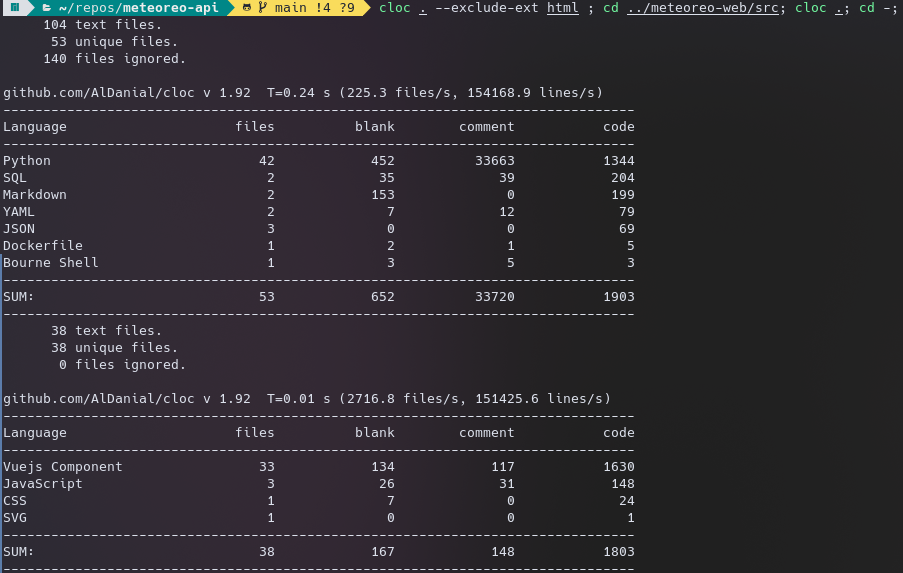
\includegraphics[width=0.8\linewidth]{images/screenshots/cloc}
%    \caption{Conteo de líneas de código.}
%    \label{fig:cloc}
% \end{figure}

\section{Sobre la extensibilidad del proyecto}

La modularidad del sistema y la forma en la que fue construído, permite que el extenderlo creando nuevos servicios sea una tarea trivial. Esto es gracias a que al ser una interfaz para ejecución de comandos, permite que las complejidades de monitoreo sean resueltas una sola vez, en la terminal de ejecución y siendo limitado sólo por la dificultad de la tarea que se busca llevar a cabo. Esto se puede ejemplificar creando un nuevo servicio de monitoreo y analizando la complejidad y el tiempo que llevan implementarlo.

Para este ejercicio, se seleccionó el crear un nuevo servicio para el monitoreo de uso de disco en las estaciones meteorológicas. Esto es importante, ya que aunque poseen un sistema de sólo lectura para asegurar la longevidad de las tarjetas SD, también cuentan con un sistema de respaldos local en memorias USB. El llevar este servicio de su concepción a un monitoreo activo, tomó aproximadamente 11 minutos, la adición de 16 líneas de código y la modificación de 2 como es posible ver en el Listado \ref{lst:git-diff-disk}. Si bien fue una tarea sencilla haciendo uso de las amplias herramientas que poseen los sistemas en los que depende, también es importante notar que el sistema de monitoreo no agergó una fricción considerable para implementarlo.

\begin{listing}
\begin{minted}[%
   breaklines
]{diff}
diff --git a/app/lib/drivers/campbell.py b/app/lib/drivers/campbell.py
-from ..services import mysql, ropi, time, weewx, proxy, campbell
+from ..services import mysql, ropi, time, weewx, proxy, campbell, disk
[...]
+    "disk": disk.service,
[...]
diff --git a/app/lib/drivers/davis.py b/app/lib/drivers/davis.py
-from ..services import mysql, ropi, time, weewx
+from ..services import mysql, ropi, time, weewx, disk
[...]
+    "disk": disk.service,
[...]
diff --git a/app/lib/services/disk.py b/app/lib/services/disk.py
+service = {
+    "command": "PERCENT=$(df /mnt/usb --output=pcent | tail -n 1 | tr -d '%')" + \
+      "if (( $PERCENT > 80 )); then echo \"true $PERCENT\"; else echo \"false $PERCENT\"; fi",
+    "stdout": "false",
+    "stderr": None,
+    "actions": {
+        "disk_almost_full": {
+            "description": "El disco está casi lleno",
+            "solution": "Elimine algunos archivos de la estación",
+            "response_stdout": "true",
+            "response_stderr": None,
+        }
+    }
+}
\end{minted}
\caption{Diferencia de código al agregar el monitoreo de disco.}
\label{lst:git-diff-disk}
\end{listing}

\section{Sobre las capacidades de carga del proyecto}

Con la ayuda de la herramienta \href{https://locust.io/}{Locust}, se realizó una prueba de estrés y carga al sistema. Esta prueba se configuró para realizar pruebas en el sistema final en el que se realizó despliegue, la prueba se compone de dos rutas a probar (véase Listado \ref{lst:locust-config}), a las cuales se les realizarán peticiones con una cantidad creciente de usuarios concurrentes. Después de haber instalado la librería, se realizaron las pruebas con el comando \texttt{locust -H http://148.210.21.98:81 -u 50 -r 0.1 -t 300s --autostart}.

Al analisar la gráfica resultante, la Figura \ref{fig:locust-graphs}, de las pruebas, es posible observar que el tiempo de respuesta incrementa de forma lineal conforme a la cantidad de usuarios, comenzando con menos de 1 segundo por respuesta e incrementando hasta alcanzar casi 50 segundos por respuesta al tener a 50 usuarios concurrentes.

\begin{listing}
\begin{minted}[%
   breaklines
]{python3}
from locust import HttpUser, task

class API(HttpUser):
    @task
    def get_drivers(self):
        self.client.get("/api/v1/drivers/")

    @task
    def get_stations(self):
        self.client.get("/api/v1/stations/",  auth=("admin", "pass"))
\end{minted}
\caption{\texttt{lcoustfile.py} configuración de pruebas.}
\label{lst:locust-config}
\end{listing}


\begin{figure}[!ht]
   \centering
   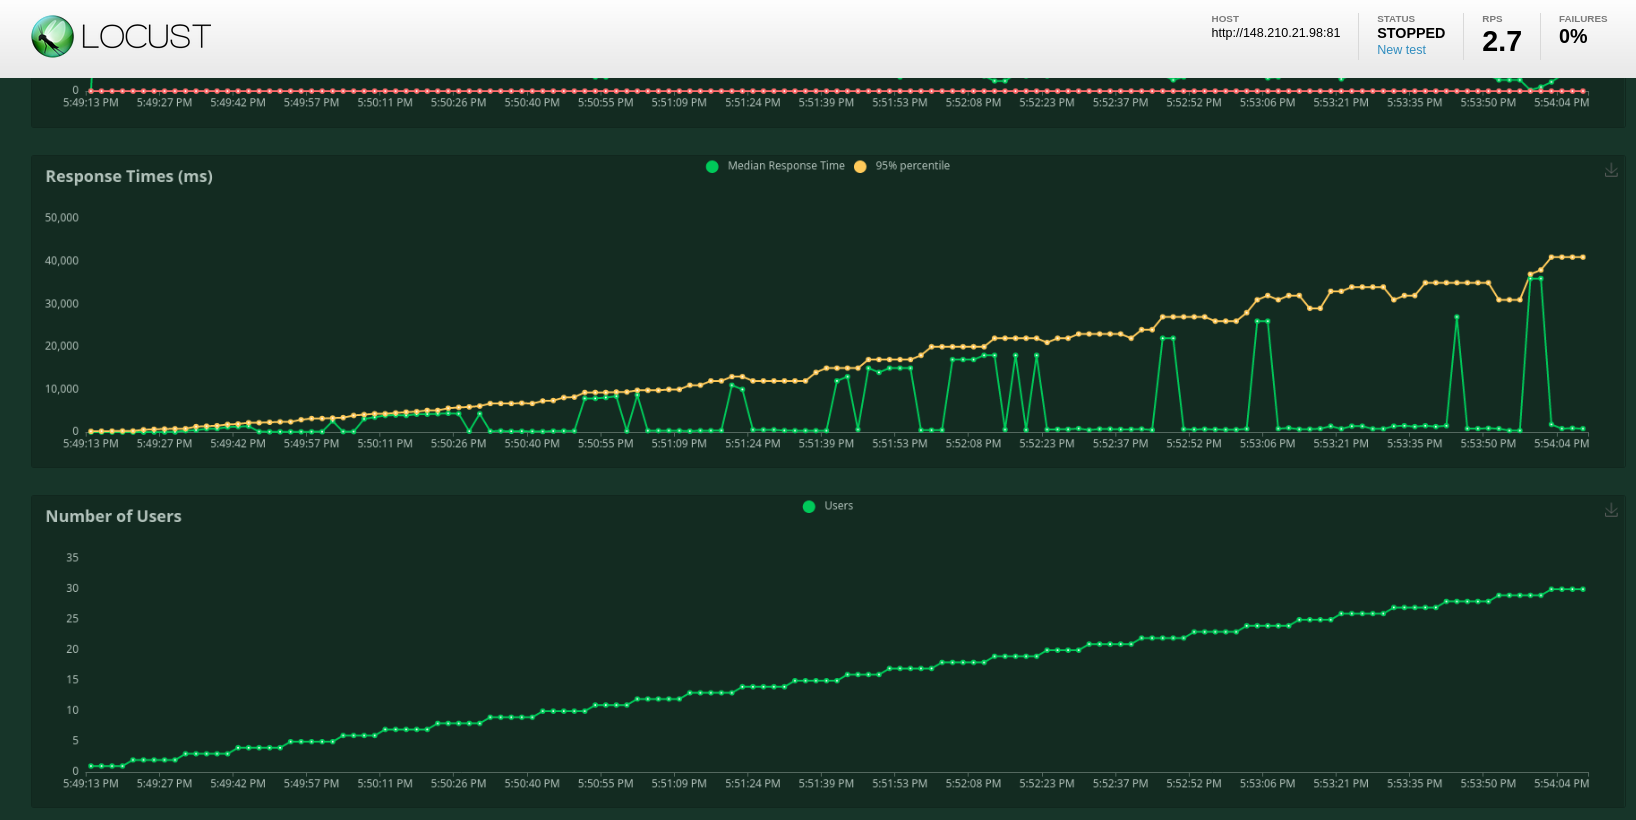
\includegraphics[width=1\linewidth]{images/screenshots/locust_graphs.png}
   \caption{Gráfica de usuarios y tiempos de respuesta creada con Locust.}
   \label{fig:locust-graphs}
\end{figure}

Sin embargo, al revisar el análisis de tiempo de respuesta por ruta presente en la Figura \ref{fig:locust-analysis}, es posible observar una diferencia significativa entre el tiempo de respuesta de la ruta \texttt{/api/v1/drivers}, con un máximo de 1.825s y la ruta \texttt{/api/v1/stations} con un máximo de 41.937s. Esto puede deberse a que la primer ruta mencionada no realiza tareas de lectura en la base de datos. Esto implicaría que la solución implementada para el almacenamiento de datos, una base de datos MariaDB en Docker en la misma máquina virtual que donde está alojado el API, no es una solución óptima para el problema.

\begin{figure}[!ht]
   \centering
   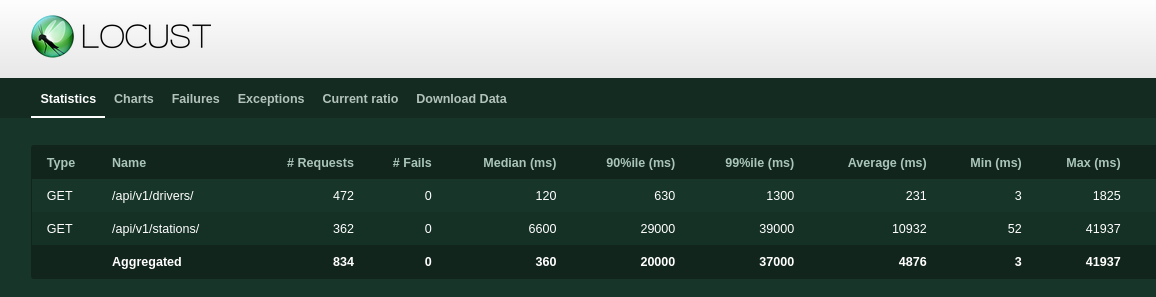
\includegraphics[width=1\linewidth]{images/screenshots/locust_analysis.png}
   \caption{Estadísticas de pruebas por ruta.}
   \label{fig:locust-analysis}
\end{figure}


\chapter{Conclusiones}\label{conclusiones}
% [Estos son los enunciados más importantes y más fuertes que se deben realizar acerca de los resultados y discusiones. Las conclusiones deben resumir el contenido y el propósito del proyecto. Se debe hacer énfasis en lo que queremos que se recuerde acerca del proyecto y realizar una síntesis de los resultados que se derivaron de los objetivos específicos trazados inicialmente (y que dieron respuesta a las preguntas de investigación si es que existen). No deben aparecer elementos nuevos o que no fueron discutidos, por ejemplo nuevos resultados observados en otros trabajos. Las conclusiones se refieren única y exclusivamente al proyecto desarrollado.

En este documento se reporta el desarrollo de un sistema de monitoreo y control para estaciones meteorológicas. A través de este apartado se presentan las conclusiones a las que se llegó durante el desarrollo del proyecto, así como las recomendaciones para trabajos futuros.

%* proyecto para titularse, decir que se aplicó lo aprendido, decir cuestiones diversas.

\section{Con respecto al objetivo de la investigación}

% Desarrollar un sistema de monitoreo y control para estaciones meteorológicas que permita un monitoreo continuo de las mismas por parte de personal no especializado, con el objetivo de proveer un mejor mantenimiento preventivo y correctivo de las estaciones meteorológicas y de calidad del aire.

%* Objetivo general entre comillas, cita textual.

Con el sistema presntado en este documento, se obtiene que es posible realizar una recolección de datos de esatciones meteorológicas y generar un sistema para la solución de problemas de forma remota. %! TODO: Terminar.

Con respecto al objetivo general del proyecto, que es el desarrollo de un sistema que permita un monitoreo continuo de estaciones meteorológicas, para proveer un mejor mantenimiento preventivo y correctivo, se logró de manera exitosa y funcional en resolver el problema descrito en la sección 1.2, conforme a los resultados presentados en el capítulo 4.


Con la realización del proyecto se lograron los siguientes resultados:

%? Desarrollar un sistema central para coordinar y recolectar los datos del estado de las estaciones.

%? Diseñar un API REST para consultar el estado de las estaciones meteorológicas.

%? Diseñar e implementar una interfaz gráfica para monitorear el estatus de las estaciones.

%? Integrar las diferentes estaciones meteorológicas existentes al sistema creando los controladores correspondientes.

%? Integrar un sistema existente de notificaciones/alertas de terceros para fallos críticos de las estaciones.
\begin{itemize}
   \item Se desarrolló un sistema para recolectar los datos del estado de las estaciones, que permitió un mejor control de la información y estado de las mismas.
   %* \item Con una recolección adecuada de los datos de la sestaciones permiten un mejor control del estado de las mismas.

   \item Se diseñó un API REST para facilitar la consulta de los datos del estado de las estaciones, documentada con OpenAPI de forma automática y,

   %* EL API REST disenado facilita la consulta del estado de las estaciones. (Se puede hacer la referencia al capítulo 3)

   \item Se generó una interfaz gráfica para la consulta del estado de las estaciones, que permitió una mejor visualización de los datos, integrado con un sistema de notificación de alertas.

   %* La interfaz gráfica permite la visualización de los datos de las estaciones de una manera más visual y sencilla.

\end{itemize}

% \section{Con respecto al futuro del proyecto}

% Por cuestiones de que las siguientes funcionalidades se encuentran fuera del alcance de este proyecto, se recomienda que sean implementadas posteriormente:

% \begin{itemize}
%    \item El utilizar un sistema automatizado para la solución de incidentes de fallos en las estaciones meteorológicas.
%    \item Generar reportes automatizados de calidad de datos y de líneas de tiempo de las estaciones con la información recolectada.
%    \item El desarrollo de un sistema de predicción de tendencias de errores, que ayude a la toma de decisiones de mantenimiento preventivo y correctivo.
% \end{itemize}

\section{Recomendaciones para futuras investigaciones}

% Debido a que las siguientes
El sistema de monitoreo de estaciones Meteoreo fué concebido como un punto de partida para más avances en el mantenimiento y monitoreo de estaciones meteorológicas. La capacidad de extensión y documentación del código tienen la arquitectura necesaria para permitir modificaciones sin alterar el funcionamiento fundamental del programa.

Actualmente, el sistema recolecta información de las estaciones meteorológicas y se permite realizar acciones en base a la información presentada, sin embargo, requiere de interacción para acciones que podrían ser automáticas. Esto abre un área de oportunidad para utilizar la información que el sistema recaba para automatizar la ejecución de las soluciones conforme a los servicios definidos, e incluso, el resolver de forma automática los errores no reconocidos en las estaciones, ya sea con una inteligencia artificial o con un sistema de pesos para una serie predefinida de soluciones comúnes.

% Se recomienda mejorar las capacidades del sistema para ser utilizado como una base de conocimientos. Entre estas se encuentra mayormente el utilizar la información de la base de datos para construir

También se recomienda el realizar un sistema de notificaciones más versátil que pueda alertar a los diferentes involucrados en la administración de las estaciones, ya que actualmente se envía una alerta de error a todos los involucrados en el sistema sin discriminar por parámetros como tipo de falla, o localización de la estación.

%! Se recomienda el que las estaciones meteorologicas se conecten al servidor para la búsqueda y ejecución de los comandos.

% Para el CECATEV se recomienda el desarrollar los controladores adecaudos para las nuevas estaciones cuando la infraestructura actual quede descontinuada, para así continuar asegurando una mayor calidad de datos.

%! Recomendaciones al laboratorio para cuando la infraestructura actual quede descontinuada.

% Fin de Conclusiones



\bibliographystyle{ieeetr}
\bibliography{referencias}


\appendix   % inician los apÈndices de la tesis

% los capÌtulos que se incluyan a partir de aquÌ aparecen
% como apÈndices
% Inicio del ApÈndice A
\chapter{Nombre del Apéndice}\label{apendiceA}

[Sustituye este texto.
En esta sección opcional se deberá incluir información secundaria o material importante que es muy extenso. El apéndice se coloca después de la literatura citada. Ejemplos de información que puede colocarse en el apéndice: una lista de universidades visitadas; los datos obtenidos de todas las repeticiones del experimento; derivaciones matemáticas extensas; todos los resultados del análisis estadístico (incluyendo quizás los no significativos) y mapas de distribución para cada fenómeno estudiado; listados completos de código fuente; etc.]

El hash del commit en Github que se entregó como producto es [HASH]


% estos comandos generan la bilbiografÌa
% La bibliografÌa se obtiene de la base de datos
% Estilos:
%	 plain (sistema numÈrico, orden alfabÈtico)
%	 unsrt (Sistema numÈrico, en el orden en que van apareciendo las citas) ------
%	 alpha (Sistema autor-fecha abreviado, orden alfabÈtico)
%	 abbrv (Sistema autor-fecha abreviado, estilo bibliogr·fico alfabÈtico abreviado)
%	 ieeepes (Bibliography Style file for articles according to IEEE instructions) Basado en unsrt



\end{document}
